%--------------------------------------------------------------------------------
% Constrói a capa com base na seção de identificação do main.tex
%--------------------------------------------------------------------------------
\begin{capa}
    \setlength{\belowcaptionskip}{0pt}
    \setlength{\abovecaptionskip}{0pt}
    \setlength{\intextsep}{-18pt}
        \begin{figure}[h]
    		\begin{center}
    		    
\includegraphics[scale=.5]{img/NEW_LOGO_UNIVASF.jpg}
    		\end{center}
    	\end{figure}

        %
\includegraphics[scale=0.6]{img/univasf.jpg}
        \center
    	{\ABNTEXchapterfont\large\imprimirinstituicao}

    	\vspace*{2cm}
    	    {\imprimirautor}
    	\vspace*{2cm}
        \begin{center}
    		\ABNTEXchapterfont\bfseries\large\imprimirtitulo
        \end{center}
    	\vfill

    	\ABNTEXchapterfont\bfseries\large\imprimirlocal\\
    	\the\year

    	\vspace*{1cm}
\end{capa}
%--------------------------------------------------------------------------------
% Constrói a folha de rosto com base na seção de identificação do main.tex
%--------------------------------------------------------------------------------
\begin{folhaderosto}
    \center
    	{\ABNTEXchapterfont\large\imprimirinstituicao}

		\vspace*{2cm}
    	    {\imprimirautor}
    	\vspace*{2cm}
		\vspace*{\fill}

		{\ABNTEXchapterfont\bfseries\large\imprimirtitulo}
		\vspace*{\fill}

		{\hspace{.45\textwidth}
		\begin{minipage}{.5\textwidth}
			\SingleSpacing
			\imprimirpreambulo \\ \\

			{\imprimirorientadorRotulo~\imprimirorientador\par}
			{\imprimircoorientadorRotulo~\imprimircoorientador\par}

		\end{minipage}%
		\vspace*{\fill}}%
		\vspace*{\fill}
			\ABNTEXchapterfont\bfseries\large\imprimirlocal\\
			\the\year
		\vspace*{1cm}
\end{folhaderosto}

%--------------------------------------------------------------------------------
% Constrói a ficha catalográfia com base na seção de identificação do main.tex
% Está comentado porque no final das contas a biblioteca do seu campus que gera a
% numeração, você pode adicionar os numeros aqui, ou anexar o pdf gerado por eles
% ao documento.
%--------------------------------------------------------------------------------
%\begin{fichacatalografica}
%	\vspace*{\fill}					% Posição vertical
%	\hrule							% Linha horizontal
%	\begin{center}					% Minipage Centralizado
%	\begin{minipage}[c]{12.5cm}		% Largura
%
%	\imprimirautor
%
%	\hspace{0.5cm} \imprimirtitulo  / \imprimirautor. --
%	\imprimirlocal, \the\year-
%
%	\hspace{0.5cm} xx p. : il. (algumas color.) ; 30 cm.\\
%
%	\hspace{0.5cm} \imprimirorientadorRotulo~\imprimirorientador\\
%
%	\hspace{0.5cm}
%	\parbox[t]{\textwidth}{\imprimirtipotrabalho~--~\imprimirinstituicao,
%	\the\year.}\\
%
%	\hspace{0.5cm}
%		1. Palavra-chave1.
%		2. Palavra-chave2.
%		I. Orientador.
%		II. Universidade xxx.
%		III. Faculdade de xxx.
%		IV. Título\\
%
%	\hspace{8.75cm} CDU 02:141:005.7\\
%
%	\end{minipage}
%	\end{center}
%	\hrule
%\end{fichacatalografica}

%--------------------------------------------------------------------------------
% Anexando a ficha catalogáfica e a folha de aprovação
%--------------------------------------------------------------------------------

\includepdf[pages=-]{anexos/ficha.pdf}

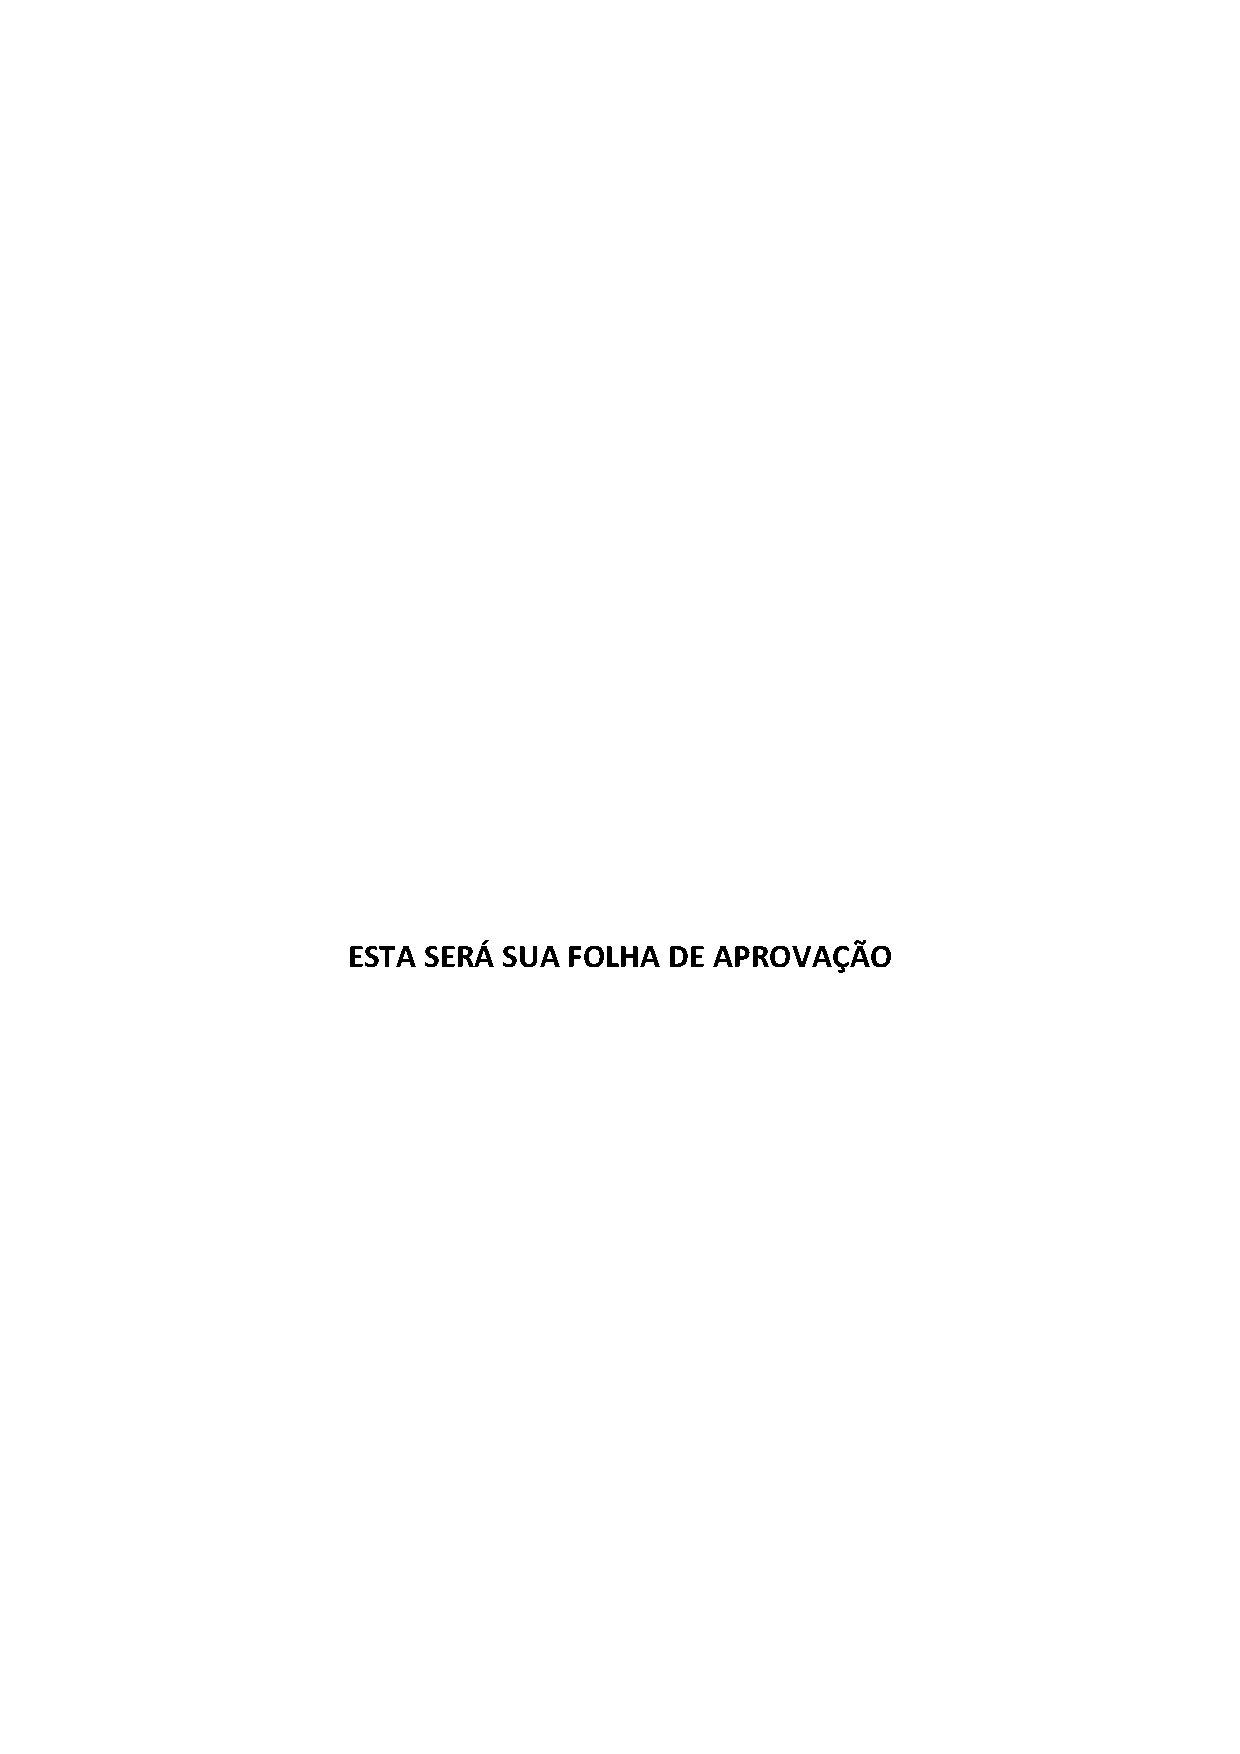
\includepdf[pages=-]{anexos/aprovacao.pdf}

\setlength{\ABNTEXsignwidth}{12cm}

%--------------------------------------------------------------------------------
% Está comentado pelo mesmo motivo da ficha catalográfica
%--------------------------------------------------------------------------------
%\begin{folhadeaprovacao}
%	\begin{center}
%	    {\ABNTEXchapterfont\bfseries\large\imprimirinstituicao}
%	    \vspace*{\fill}
%
%	    {\ABNTEXchapterfont\bfseries\large FOLHA DE APROVAÇÃO}
%	    \vspace*{\fill}
%
%	    {\ABNTEXchapterfont\bfseries\large\imprimirautor}
%
%	    \vspace*{\fill}\vspace*{\fill}
%	    {\ABNTEXchapterfont\bfseries\large\imprimirtitulo}
%	    \vspace*{\fill}
%
%	    {\hspace{.45\textwidth}
%		\begin{minipage}{.5\textwidth}
%			\SingleSpacing
%			\ABNTEXchapterfont\imprimirpreambulo \\ \\
%
%			{\ABNTEXchapterfont\imprimirorientadorRotulo~\imprimirorientador\par}
%			{\ABNTEXchapterfont\imprimircoorientadorRotulo~\imprimircoorientador\par}
%
%		\end{minipage}%
%	    \vspace*{\fill}}
%	\end{center}
%
%	\vspace*{\fill}
%
%	\begin{center}
%			 \ABNTEXchapterfont\large Aprovado em: \_\_\_\_ de \_\_\_\_ de 2017
%	\end{center}

%	\vspace*{\fill}

%	\begin{center}
%			 \ABNTEXchapterfont\bfseries\large Banca Examinadora
%	\end{center}
%
%   \ABNTEXchapterfont\assinatura{Fábio Nelson de Sousa Pereira, Mestre, Universidade Federal do Vale do São Francisco}
%	\ABNTEXchapterfont\assinatura{Jorge Luis Cavalcanti Ramos, Doutor, Universidade Federal do vale do São Francisco}
%  \ABNTEXchapterfont\assinatura{Ricardo Argenton Ramos, Doutor, Universidade Federal do Vale do São Francisco}
%	 \vspace*{\fill}


%\end{folhadeaprovacao}

%--------------------------------------------------------------------------------
% Insere a epígrafe
%--------------------------------------------------------------------------------
\newpage
\vspace*{\fill}
\begin{flushright}
		\textit{“A persistência é o caminho do êxito.”}
		\textbf{Charles Chaplin}
\end{flushright}

%--------------------------------------------------------------------------------
% Seção de agradecimentos
%--------------------------------------------------------------------------------
\begin{agradecimentos}

Agradeço a mim, por não desistir;

Agradeço a Deus, por me dar forças;

Ao meu orientador Professor Mestre e em breve Doutor Juracy Magalhães, compreensivo e paciente, me deu as ferramentas para chegar ate aqui.

Agradeço também aos meus pais, meus irmãos e família, que sempre investiram em mim e confiaram no meu potencial. Agradeço à minha namorada que tanto me incentivou e acreditou em mim. Também quero agradecer aos amigos e colegas que forneceram bons momentos de descontração.

Fico feliz por ter boas pessoas ao meu redor que querem me ver vencendo os desafios da vida! Gratidão.


\end{agradecimentos}

%--------------------------------------------------------------------------------
% Insere a segunda epígrafe
%--------------------------------------------------------------------------------
\begin{epigrafe}
    \vspace*{\fill}
	\begin{flushright}
		Se pude enxergar a tão grande distância, foi subindo nos ombros de gigantes.\\
		 \vspace{\baselineskip}
		\textbf{Isaac Newton}\\
		\textbf{Carta à Robert Hooke, 1676}
	\end{flushright}
\end{epigrafe}



%--------------------------------------------------------------------------------
% Seção de resumos
%--------------------------------------------------------------------------------
% resumo em português
\setlength{\absparsep}{18pt} % ajusta o espaçamento dos parágrafos do resumo
\begin{resumo}

     O estudo da modelagem e simulação do manipulador robótico EEZYBotArm através das ferramentas CoppeliaSim e Robotics Toolbox para Phython (RTB) envolve a cultura Maker, que está firmemente estabelecida e cresce impulsionada pela filosofia do "faça-você-mesmo", e que entre os projetos frequentes nesse movimento, destacam-se os braços robóticos. O propósito deste estudo é realizar a modelagem e simulação de um manipulador robótico fruto da cultura Maker utilizando as ferramentas CoppeliaSim e Robotics Toolbox. Esses manipuladores apresentam várias configurações, incluindo os antropomórficos com geometria em paralelogramo, caracterizados por cadeias fechadas, arquitetura que proporciona alta capacidade de carga, precisão nos movimentos e mantém o efetuador sempre paralelo ao solo, vantajoso para tarefas de paletização. Além disso, no desenvolvimento de manipuladores robóticos, a análise cinemática é de suma importância. A utilização de ferramentas computacionais como simuladores e bibliotecas de ferramentas (toolboxes) torna-se essencial para modelar, visualizar e calcular a cinemática (e dinâmica), particularmente no contexto de braços robóticos com geometria em paralelogramo. Para isso, o modelo virtual do protótipo foi construído no CoppeliaSim, e no RTB foi proposto analisar cineticamente esse manipulador de cadeia fechada para computar os ângulos de junta, estabelecendo comunicação entre essas duas ferramentas para visualizar o resultado no modelo virtual. Ao final deste trabalho, a adoção de um modelo amador e sua modelagem no ambiente de simulação CoppeliaSim e a subsequente análise da cinemática inversa com uso de ferramentas e bibliotecas em Python (uma linguagem de programação) foi bem sucedida, oferecendo esclarecimentos valiosos para o desenvolvimento de modelos semelhantes, e também facilitando a implementação desses modelos em contextos acadêmicos e educacionais, promovendo uma maior interação com a robótica. 
	

 \textbf{Palavras-chave}: \textit{Robótica. Simulação. Modelagem. CoppeliaSim. Manipulador Robótico. Cadeia fechada.}

\end{resumo}

%---------------------------------------------------------------------------------
% resumo em inglês
\begin{resumo}[Abstract]
\begin{otherlanguage*}{english}

	The study of the modeling and simulation of the EEZYBotArm robotic manipulator using the CoppeliaSim and Robotics Toolbox for Phython (RTB) tools involves the Maker culture, which is firmly established and growing, driven by the "do-it-yourself" philosophy, and among the frequent projects in this movement, robotic arms stand out. The purpose of this study is to model and simulate a robotic manipulator resulting from the Maker culture using the CoppeliaSim and Robotics Toolbox tools. These manipulators come in various configurations, including anthropomorphic ones with parallelogram geometry, characterized by closed chains, an architecture that provides high load capacity, precision in movements and keeps the effector always parallel to the ground, which is advantageous for palletizing tasks. Furthermore, in the development of robotic manipulators, kinematic analysis is of utmost importance. The use of computational tools such as simulators and toolboxes is essential for modeling, visualizing and calculating kinematics (and dynamics), particularly in the context of robotic arms with parallelogram geometry. To this end, the virtual model of the prototype was built in CoppeliaSim, and in RTB it was proposed to kinetically analyze this closed-chain manipulator to compute the joint angles, establishing communication between these two tools to visualize the result in the virtual model. At the end of this work, the adoption of an amateur model and its modeling in the CoppeliaSim simulation environment and the subsequent analysis of the inverse kinematics using tools and libraries in Python (a programming language) was successful, offering valuable insights for the development of similar models, and also facilitating the implementation of these models in academic and educational contexts, promoting greater interaction with robotics. 
	

	\vspace{\onelineskip}

	\noindent
	\textbf{Palavras-chave}: \textit{Robotics. Simulation. Modeling. CoppeliaSim. Robotic manipulator. Closed chain.}

\end{otherlanguage*}
\end{resumo}


%---------------------------------------------------------------------------------
% Insere lista de ilustrações
%---------------------------------------------------------------------------------
\begin{KeepFromToc} % Este comando evita que todas as seções dentro dele de apareçam no sumário
\pdfbookmark[0]{\listfigurename}{lof}
\listoffigures
%\addcontentsline{toc}{chapter}{Lista de Figuras}
\cleardoublepage


%---------------------------------------------------------------------------------
% Insere lista de tabelas
%---------------------------------------------------------------------------------
\pdfbookmark[0]{\listtablename}{lot}
\listoftables
\cleardoublepage

%---------------------------------------------------------------------------------
% Insere lista de quadros
%---------------------------------------------------------------------------------
%\pdfbookmark[0]{\listofquadrosname}{loq}
%\listofquadros*
%\cleardoublepage

%---------------------------------------------------------------------------------
% Ajusta lista de código - alterar de figures para códigos - by @Gabrielr2508
%---------------------------------------------------------------------------------
\makeatletter
\let\l@listing\l@figure
\def\newfloat@listoflisting@hook{\let\figurename\listingname}
\makeatother

%---------------------------------------------------------------------------------
% Insere lista de códigos - by @leolleocomp
%---------------------------------------------------------------------------------
\listoflistings


%---------------------------------------------------------------------------------
% Insere lista de abreviaturas e siglas
%---------------------------------------------------------------------------------
\begin{siglas}
	\item[DIY]       Do it yourself
    \item[DH]		 Denavit-Hartenberg
    \item[MDH]		 Modified Denavit-Hartenberg
    \item[RTB]		 Robotics Toolbox
    \item[ROS]       Robot Operating System
    \item[VANTs]     Veículos Aéreos Não Tripulados
	
\end{siglas}
\end{KeepFromToc}

%---------------------------------------------------------------------------------
% Insere o sumario
%---------------------------------------------------------------------------------
\pdfbookmark[0]{\contentsname}{toc}
\tableofcontents*
\cleardoublepage


